\singlechapter{Hockey \label{chap:hockey}}

Attention must be drawn to the safety of the players and spectators.
Thus, the safety rules have to be obeyed strictly and all equipment must be in good condition.
These rules cannot cover every situation.
Teams have to agree on a specific amount of elbow-room before playing.
The different backgrounds of the players and the conditions of the location have to be considered.
Fairness of everyone involved is vital.

\section{Playing Field}

\subsection{Dimensions}

\begin{figure}[h]
\begin{center}
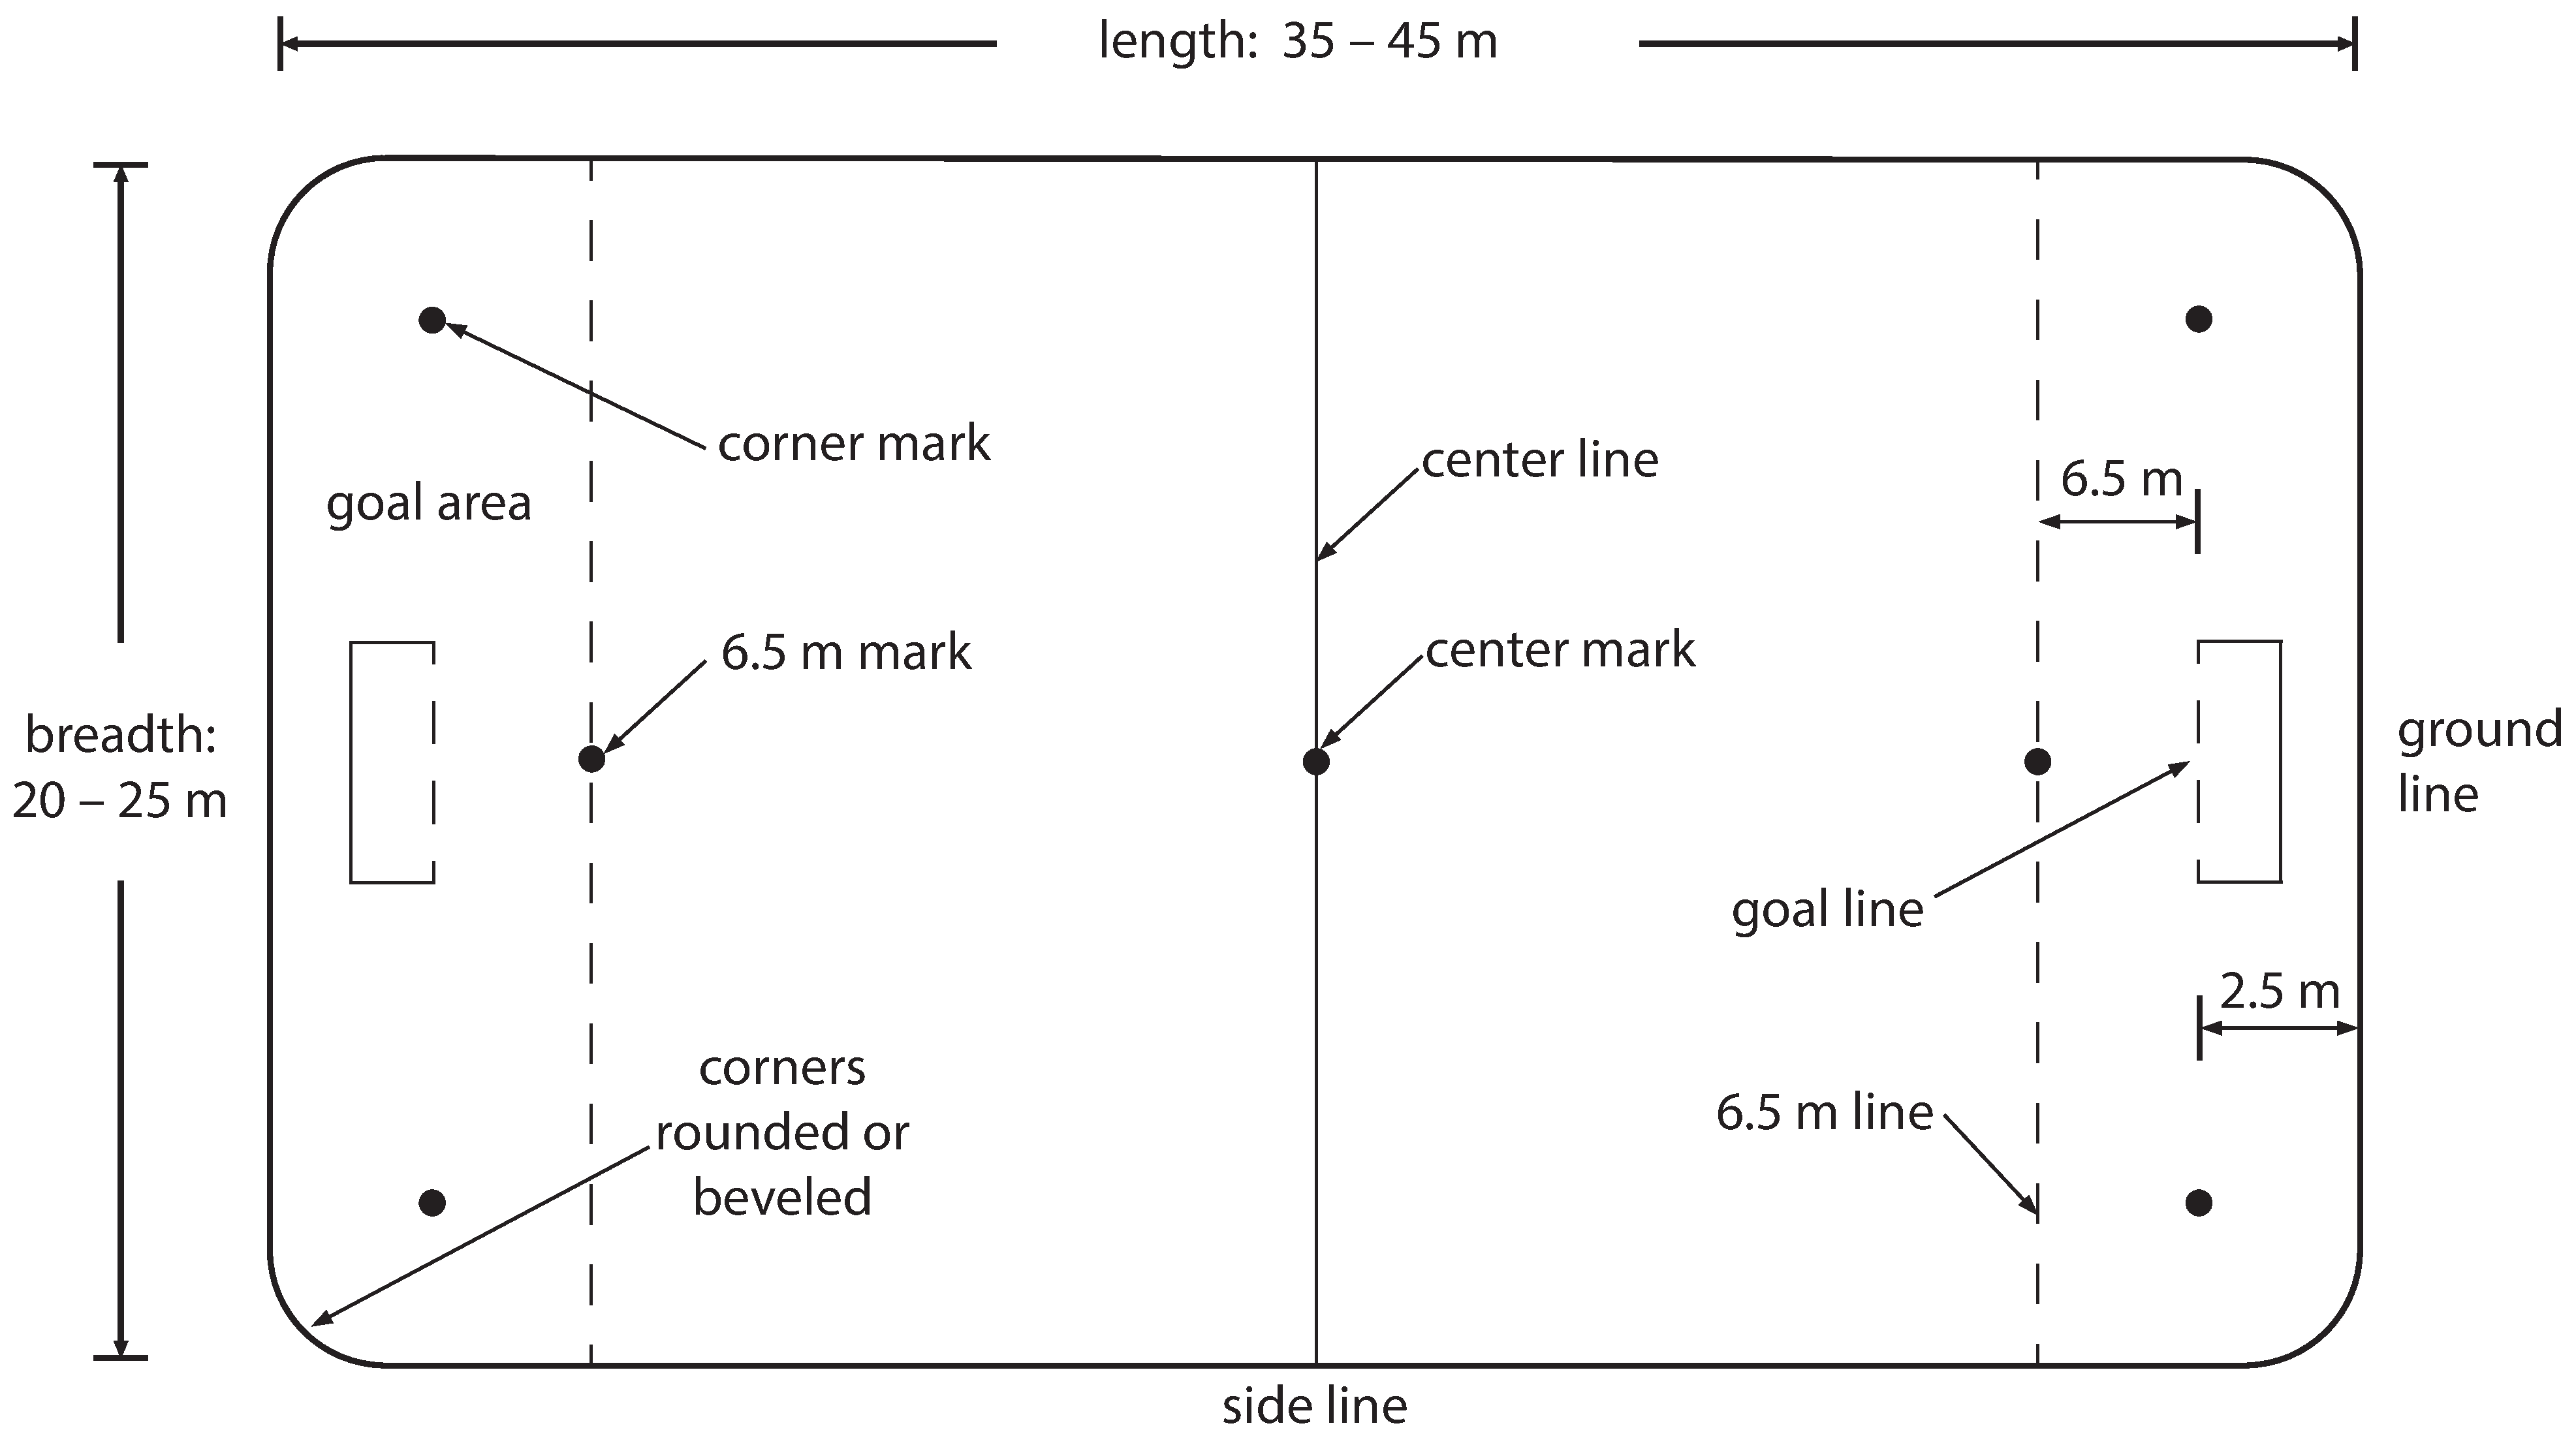
\includegraphics[scale=0.22]{dimension}
\end{center}
\end{figure}

\subsection{}
The field has a length of 35 to 45 meters and a breadth of 20 to 25 meters.
It is surrounded by barriers.
The corners are rounded or beveled.

\subsection{Goals}
The posts are 2.50 m in from the ends of the playing field (ground lines), ensuring that the players can go behind them.
The inside dimensions of goal openings are 1.20 m high and 1.80 m wide.
The goals must be made in such a way that the ball cannot enter through the rear or sides. The goals must not have sharp, pointed or protruding parts.

\subsection{Markings}
The center line divides the field into two equal halves, and the center mark is in the middle of the center line.
There are marks in front of each goal at a distance of 6.5 m.
The goal lines connect the posts on the ground.
The corner marks are on the extension of the goal lines, 1.0 m in from each side line.
The 6.5 m lines are parallel to the goal lines and run through the 6.5 m marks.
The goal areas are between the 6.5 m lines and the ends of the field.

\section{Teams}

\subsection{Number Of Players}
A team consists of five players (plus substitutes).
Substituting one player for another is possible at any time.
It is not necessary to indicate it to the Referee.
The new player must enter the field where the other exits it.
Each player can be the goalkeeper at any time.
The goalkeeper has no special rights.
To take part in a game, a team must have at least three players.

\section{Clothing}
Shoes must be worn.
All players of a team must wear shirts of the same color.
The color must be clearly different from the opponent's color.
At tournaments and other large events each team should have two different colored sets of shirts.

Clothing suggestions for comfort and safety:
\begin{itemize}
\item Cycling shorts and kneepads, or long pants
\item Gloves
\item Short shoe laces, or laces tucked in
\item Helmet and dental protection
\item Definitely no jewelry (watches, necklaces, earrings)
\end{itemize}

\section{Equipment}

\subsection{Unicycles}
The maximum wheel size is 618mm (24$"$).
The unicycles must not have sharp or protruding parts anywhere that might cause injuries.
This refers especially to quick-release levers and bolts.
The pedals must be plastic or rubber.

\subsection{Sticks}
All sticks legal for playing ice-hockey or floorball (apart from those for the goalkeeper) can be used.
Cracked or splintered sticks must be taped or repaired before play.
An upper end made of rubber is recommended.

\subsection{Ball}
A ``dead'' tennis ball that reaches 30 percent to 50 percent of its original height after bouncing onto concrete is used.
Alternatively, a street hockey ball can be used.
The choice is made by the hosting organization if the opposing teams do not agree on which ball to use.
The chosen type of ball must be announced well in advance of the competition, and must be obtainable in all participating countries.

\section{Penalties}
In every instance of a violation of the rules the Referee must penalize the offending team, unless the Referee decides not to interrupt the game (advantage).

\subsection{Free Shot}
The free shot is the standard penalty for all violations of the rules.
It is applied in all cases except for those explicitly mentioned in sections \ref{subsec:hockey_penalties_65m}–\ref{subsec:hockey_penalties_bully}.
The free shot is executed from the point where the violation was done.
\textbf{Exceptions}: If a team gets a free shot within the opponents' goal area, the free shot is done from the closest corner mark (corner shot).
If a team gets a free shot within their own goal area, the free shot is done at a distance of 1 m in front of the goal line (goalkeeper's ball).
The free shot is indirect.
The player executing the free shot may only touch the ball once.
Then another player has to touch the ball.
Opposing players must keep a distance with their unicycles and their sticks of at least 2.0 m from the ball.

\subsection{6.5 M \label{subsec:hockey_penalties_65m}}
If legal playing would have led to a direct chance to score a goal, a ``6.5 m'' is given.
This includes fouls outside the goal area.
The ball is placed at the 6.5 m mark.
A player of the defending team goes to the goal and must sit with the bottom of the wheel of their unicycle within 0.5 m of the goal line.
The other team chooses a player to shoot the 6.5 m.
All other players must leave the goal area.
After the Referee's whistle the goalkeeper must ride the unicycle freely and not rest on the goal.
If no goal is scored, play continues as soon as the ball touches the post, the keeper touches the ball or the ball crosses the extended goal line.

\subsection{Penalty Goal}
If the defending team prevents a goal from being scored through an illegal play of the ball and if, in the opinion of the Referee, the ball was traveling directly toward the goal and would definitely have entered the goal without being touched by another player, a penalty goal may be awarded.
In this case the attacking team is awarded a goal.
If there is any doubt as to the certainty of a goal, a 6.5 m must be awarded as described in section \ref{subsec:hockey_penalties_65m}.

\subsection{Bully \label{subsec:hockey_penalties_bully}}
Whenever the game needs to be resumed without penalizing one of the teams, this is done with a bully (face off).
For the bully, the Referee drops the ball between two opposing players.
Playing starts when the ball touches the ground.
A bully during the game is executed where the ball was when the game was interrupted. 
Exception: Within the goal area, the bully is always executed near one of the corner marks.

\subsection{Penalty Box}
The Referee can send a player off the field for two minutes, five minutes or for the remainder of the game.
This is done in the case of unsporting behavior and also for intentional or dangerous disregard of the rules.
While a player is in the penalty box, the team may not substitute a replacement for that player.

\section{Course Of The Game}

\subsection{Game Duration}
The play time is given by the playing schedule.
It is a relative play time.
The time only stops if the Referee requests a time out.
The teams change sides during the break.
At the start of each period, all players must be in their own half of the field.
Each period starts with a bully at the center mark.
If the game ends in a draw and a decision is necessary, play is continued for ten more minutes: five-minute break and change sides, five minutes of play, change sides without a break and five more minutes of play.
If it's still a draw, a decision is reached with a penalty shootout.

\subsection{Penalty Shootout}
Three of the players from each team get one penalty shot each.
If it is still a draw, each team shoots one more penalty until there is a decision.
It is possible that one player can make more than one shot.
However, in all cases at least two other players have to make a shot before the same player can shoot again.

For the penalty, all players except for a defending goalkeeper leave the corresponding half of the playing field.
The goalkeeper must be close to the goal line, at least until the attacking player has had contact with the ball.
The Referee places the ball on the center point and the player taking the shot will, after the whistle of the Referee, play the ball from there, trying to score a goal.
The ball must be kept in motion towards the goal line (no backwards movement allowed) and once it is shot, the play shall be considered complete.
No goal can be scored on a rebound of any kind (an exception being the ball off the goal post, then the goalkeeper and then directly into the goal), and any time the ball crosses the goal line, the shot shall be considered complete.

\subsection{Riding The Unicycle}
The player has to be riding the unicycle freely.
He or she may use the stick as support but must not rest on the goal or the wall or something similar.
It is not sufficient to release the goal only quickly for the time while the goalkeeper takes part in the game.
A short support on the wall to avoid a dismount can be tolerated.
A player who is falling off the unicycle may take part in the game until touching the ground.
A remounting player must sit on the seat and have both feet on the pedals before participating in the game again.
If a player who is not riding a unicycle shoots into their own goal, the advantage rule applies for the attacking team and the goal is valid.

\subsection{Obstacle}
A player who is off the unicycle must not be an obstacle for opponents.
The player is considered an obstacle if the player, the unicycle or stick is hit by the ball and also if an opponent cannot move around freely.
The player should remount at the same spot, but if necessary move out of the way of play first.

\subsection{Contact With The Ball}
The stick, the unicycle and the whole body can be used to play the ball.
It all counts as a contact.
Players are allowed to play the ball with the body twice in a row only if one of the contacts is passive.
When the ball is played with the body, the player must not catch or otherwise hold the ball and the contact with the ball should be instantaneous.
For arms and hands see also section \ref{subsec:hockey_goal-shots_with-arms-or-hands}.

\subsection{Start and Stop}
Starting and resuming the game is always initiated by the Referee's whistle.
When the Referee blows the whistle during the game, it is interrupted immediately.

\subsection{Restart After A Goal}
After a goal, the non-scoring team gets the ball.
All players must go to their own half.
After the Referee's whistle, the game resumes when the ball or a player of the team in possession crosses the center line.
It is legal to directly shoot a goal after passing the center line, for example without passing the ball to another player first.

\subsection{Ball Out Of Bounds}
If the ball leaves the field, the team opposite to that of the player who last touched it gets a free shot or a corner shot, depending where the ball went out.
The free shot is done 1.0 m in from the side line.

\subsection{Moving The Goal}
If a player moves the goal, the game is interrupted and the opposing team gets a free shot.

\subsection{Ball In Spokes}
If the ball gets stuck between the spokes of someone's unicycle, the opposing team gets a free shot (not a 6.5m penalty).

\section{Fouls}

\subsection{General Considerations}
All players must take care not to endanger others.
The game is contactless: the opponents and their unicycles may not be touched.
The players must take care not to hit an opponent with their stick, especially after a shot.
Only in the vicinity of the ball, they may touch an opponent's stick with their stick to block them.
However, this contact may not be hard.
It is illegal to turn the blade of the stick upside down in order to hook into an opponent's stick.
Raising the opponent's stick is allowed in principle, if not done using exaggerated roughness.
If the opponent's stick is raised above the height of their hips, it is always considered exaggerated roughness.

\subsection{Right Of Way}
To keep the game going, rule violations that do not influence the course of the game should not be penalized.
The following rules apply when riders come into contact with each other:
\begin{itemize}
\item No player may endanger another player by forcing them to give way (for example, to push them toward the wall).
\item A player who is idling or resting on the stick must be evaded.
\item The leading of two players riding next to each other may choose the direction of turns. If both are evenly side-by-side, the one having the ball may choose the direction.
\item If two players are approaching each other directly or at an obtuse angle, the one with the ball has the right of way.
\item In all cases not mentioned above, it is up to the Referee to make a decision.
\end{itemize}

\subsection{SUB (Stick Under Bike)}
A player who holds his or her stick in a way that someone else rides over or against it is committing a foul, regardless of intention.
According to the situation the player who was ``subbed'' is given either a free shot or a 6.5 m.

\subsection{SIB (Stick In Bike)}
If a stick gets into the spokes of an opponent, the holder of the stick is committing a foul regardless of intention.
According to the situation the player who was ``sibbed'' is given a free shot or a 6.5 m.

\subsection{Insults}
A player must not insult the Referee or other players.

\subsection{Intentional Fouls \label{subsec:hockey_fouls_intentional-fouls}}
Intentional fouls are considered to be unsporting behavior.
The respective player is sent off the field for at least 2 minutes.

\section{Goal Shots}

\subsection{Goal Shot With Arms Or Hands \label{subsec:hockey_goal-shots_with-arms-or-hands}}
A goal is disallowed if scored with arms or hands.
The defending team gets a free shot (goalkeeper's ball).
This rule does not apply if the ball is shot into one's own goal.

\subsection{Long Shot}
A goal is disallowed if the last contact with the ball was made when the ball was in one's own half.
The defending team gets a free shot (goalkeeper's ball).
This rule does not apply if the ball is shot from the opponents' half into one's
own goal.

\subsection{Ball In The Outside Of The Net}
If the ball becomes lodged in the outside of the goal net, or if the ball entered the goal through the net from the side the back through a hole in the net, a free shot is given against the team whose player last played the ball.

\section{Safety Rules}

\subsection{Throwing Sticks}
A player who intentionally drops or throws his or her stick is sent off the field for at least 2 minutes, at the discretion of the Referee (section \ref{subsec:hockey_fouls_intentional-fouls}).
Also, the opposing team gets a 6.5 m.

\subsection{Top Of The Stick}
The upper end of the stick must always be covered with one hand to avoid injury to other players.
A brief removal of the upper hand from the stick to play the ball with that hand is acceptable provided that this is done in a safe manner.

\subsection{The Lower End Of The Stick}
The lower end of the stick must always be below the players' hips to avoid injury to other players.
\textbf{Exception:} In direct vicinity of one's own goal, the lower end of the stick can be raised as high as the crossbar of the goal.

\subsection{Exaggerated Roughness}
Exaggerated roughness can lead to injuries and must therefore be avoided.

\section{Referee Rules}

 \subsection{Members Of The Board Of Referees}
\begin{wrapfigure}{r}{0.5\textwidth}
\begin{center}
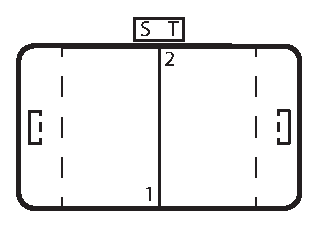
\includegraphics[scale=0.75]{referees}
\end{center}
\end{wrapfigure}
 The Board of Referees consists of:
\begin{itemize}
\item First Referee (1) 
\item Second Referee (2)
\item Secretary (S)
\item Timer (T)
\end{itemize} 

\subsection{The Referees}
The two Referees are positioned one on each side.
They try to stay close to the ball.
They should not ride a unicycle.
The clothes of the Referees must be of different color than those of the players.
Both Referees are responsible for checking all violations of the rules.
The first Referee has three additional tasks:
\begin{itemize}
\item The First Referee overrules the Second Referee, if they disagree.
\item The First Referee restarts the game after every interruption by a long blow of the whistle.
\item The First Referee drops the ball in for the bully.
\end{itemize}

\subsection{The Secretary}
The Secretary sits at the desk and takes care that the scoreboard always shows the current score.
After a goal the Secretary seeks eye contact with the First Referee to check if the goal is declared valid or not.
After the end of the game the Secretary writes the final score into the report.

\subsection{The Timer}
The Timer checks the time of play with a stopwatch.
The watch is started whenever the Referee starts the game by blowing the whistle.
At the end of each period, the Timer stops the game by blowing the whistle.
The Timer also stops the time whenever the Referee requests a time out.

\subsection{Before The Game}
Before the game, the Referees assemble all players on the field (including substitutes).
They check the following:
\begin{itemize}
\item Are the colors of the shirts of the players clearly different?
\item Did all players take off their watches and jewelry that might injure others?
\item Is the ball suitable?
\item Are the unicycles and sticks orderly, without sharp, pointed or protruding parts that might injure others?
\item They explain to the players how strictly they will interpret the rules.
\item If necessary, they tell the players how long the game will be and also if there is extended time in case of a draw.
\end{itemize}

\subsection{General}
The game is interrupted by a short and loud blow of the whistle.
If any players don't hear the whistle, it is necessary to blow the whistle again.
It is not possible to let the game continue after blowing the whistle.

The Referees should set the tone through their positive and calm appearance.
Decisions are explained upon request but they are not discussed with the players.
In an unclear situation, the Referees can ask the players before making a final decision.

Neither the Referees nor the Timer or Secretary may be distracted from the game.
Most of all, they must not talk with the spectators during the game.

If two violations of the rules occur back-to-back, only the first one is penalized.
Exception: Unsporting behavior should be penalized even after the game has been interrupted.

After a goal, the Referee waits until both teams are back in their own halves and ready to continue.
Only then, the first Referee starts the game by blowing the whistle.

If the teams start to play even though the game had not been started by the Referee, it is stopped immediately by two or more quick consecutive blows of the whistle.

To apply the advantage rule, the Referee makes the normal sign for a free shot with one arm pointing in the direction of play of the team who has the advantage.
In addition, the Referee may shout ``Advantage'' or ``Go ahead!'', but does not blow the whistle.
The end of advantage play should be signified, either by blowing the whistle to give a free shot for the original foul in the case where no advantage was gained, or by lowering the arm again and/or shouting ``Advantage over''.

After each interruption of the game the Referee briefly explains the decision.
In addition the corresponding hand sign is shown.

When two or more players fall and it is unclear whether a foul occurred, the Referees can interrupt the game and then continue it with a bully.
This prevents that even more players are drawn into the situation.

The Referees suspend the game if an injury occurs.
Afterwards, a free shot is given to the team that was in possession of the ball at the time of the interruption.
If it is unclear who was in possession, the game is continued with a bully.

\subsection{Referee Hand Signs}
\renewcommand{\arraystretch}{1.5}
\begin{longtable}{|p{3cm}|p{11cm}|}

\hline
\raisebox{-1\height}{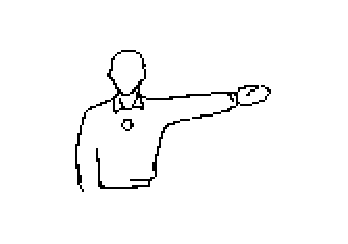
\includegraphics[scale=0.6]{1_h}}
&
\textbf{``Free shot''}

Point with the extended arm in the direction of play.

This sign is also used to indicate the advantage rule. \\
\hline
\raisebox{-1\height}{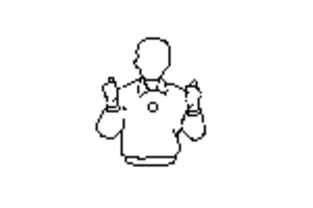
\includegraphics[scale=0.6]{2_h}}
&
\textbf{``Bully''}

Hold both thumbs up.  \\
\hline
\raisebox{-1\height}{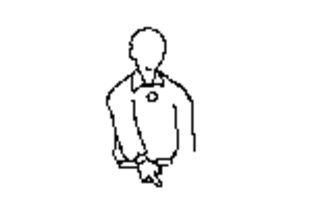
\includegraphics[scale=0.6]{3_h}}
&
\textbf{``6.50 m''}

Point with the index finger to the 6.50 m point. \\ 
\hline
\raisebox{-1\height}{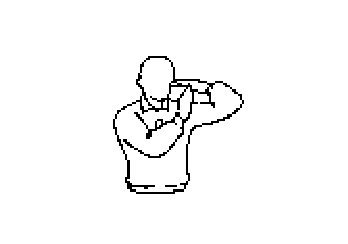
\includegraphics[scale=0.6]{4_h}}
&
 \textbf{``No Foul''}

Extend both arms horizontally.

This sign is used to indicate that there was no foul in a critical situation. It is not used in conjunction with a blow of the whistle. \\ 
\hline
\raisebox{-1\height}{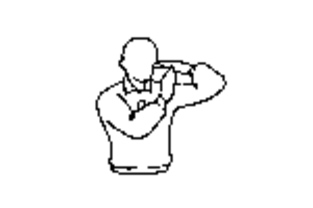
\includegraphics[scale=0.6]{5_h}}
&
\textbf{``Time out''}

Form the letter ``T'' with both hands.

The game is interrupted for example if a player is injured or if the spectators disturb the game. \\ 
\hline
\raisebox{-1\height}{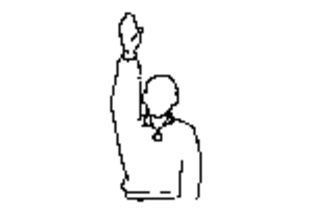
\includegraphics[scale=0.6]{6_h}}
&
\textbf{``Goal''}

Point upwards vertically with one arm.

The Referees should check here that the secretary notes the goal.
To control this it may be useful for the Referees to write down the score themselves. \\ 
\hline
\raisebox{-1\height}{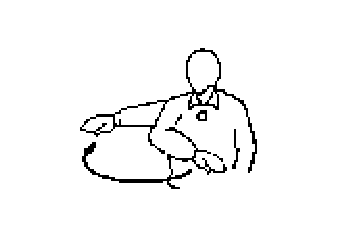
\includegraphics[scale=0.6]{7_h}}
 &
 \textbf{``No goal''}

Move the flat hand horizontally (palm pointing down).

With this hand sign a goal shot is declared invalid.
This is for example the case if the ball was last touched by hand or arm, in case of a long shot, if the ball entered the goal through the net from the outside, or if the game had already been stopped before the ball entered the goal.
The referees should check here that the Secretary does not inadvertently count the invalid goal.\\ 
\hline
\raisebox{-1\height}{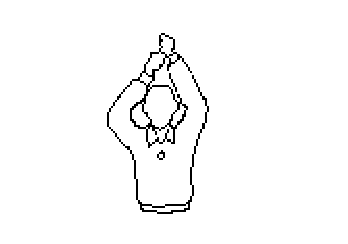
\includegraphics[scale=0.6]{8_h}}
&
\textbf{``High stick''}

Hold clenched fists next to each other above the head. \\ 
\hline
\raisebox{-1\height}{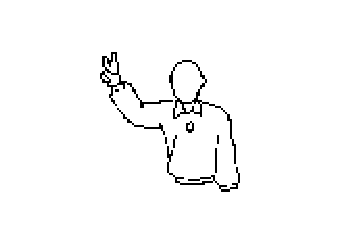
\includegraphics[scale=0.6]{9_h}}
&
\textbf{``Penalty box for 2 minutes''}

and also 

\textbf{``Two consecutive plays with the hand''}

Spread and raise two fingers.  \\ 
\hline
\raisebox{-1\height}{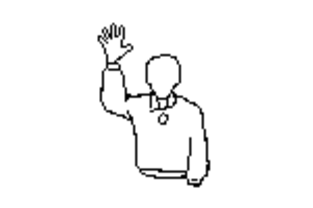
\includegraphics[scale=0.6]{10_h}}
  &
\textbf{``Penalty box for 5 minutes''}

Spread and raise five fingers.\\
\hline
\end{longtable}
\renewcommand{\arraystretch}{1}